\section{Tập chuẩn và đa hộp}
\begin{dn} [Tuy2000 \cite{Tuy2000}]
Một tập $Q \subset \R^p_+$ được gọi là một tập chuẩn (normal set) nếu với mọi $q \in \R^p_+$, ta có
\begin{equation*}
    q \in Q \Rightarrow (q - \R^p_+) \cap \R^p_+ \subseteq Q \text{.}
\end{equation*}
\end{dn}

\begin{vd}
Từ định nghĩa trên ta thấy $\empty, \{0\}, \R^p_+$ đều là các tập chuẩn. Hình \ref{fig:1} là ví dụ cho một tập chuẩn trong không gian hai chiều.
\end{vd}

\begin{md}[Tuy2000 \cite{Tuy2000}]
     Nếu $Q$ là một tập chuẩn thì $ Q \cup \{q \in R^p_+ | q_i = 0, i \in \{1, . . . , p\}\}$ cũng là một tập chuẩn.

\end{md}

\begin{dn} [Tuy2000 \cite{Tuy2000}]
    Một tập $Q \subset \R^p_+$ được gọi là một \textit{tập chuẩn đảo (reversed normal set)} nếu với mọi $q \in \R^p_+$, ta có
    \begin{equation*}
        q \in Q \Rightarrow q + \R^p_+ \subseteq Q \text{.}
    \end{equation*}
\end{dn}
Cho $0 \leq d, Q \subseteq [0, d]$ được gọi là một tập chuẩn đảo trong hộp $[0, d]$ nếu với mọi $q \in [0, d]$, ta có
\begin{equation*}
    q \in Q \Rightarrow (q + \R^p_+) \cap (d - \R^p_+) \subseteq Q.
\end{equation*}

\begin{figure}[!h]
    \centering
    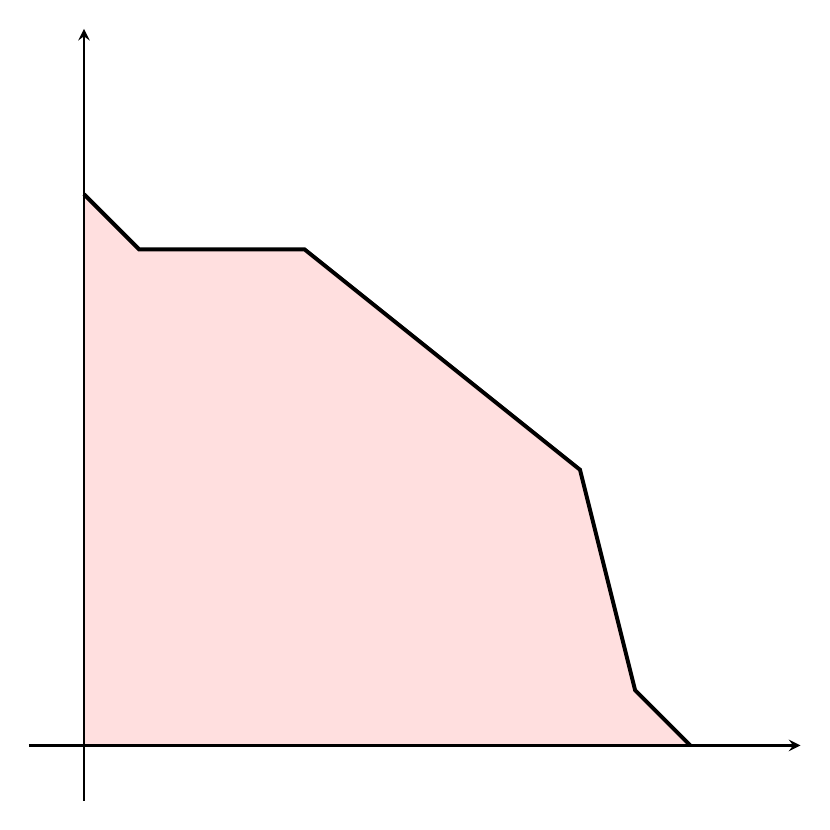
\begin{tikzpicture}[
        > = stealth, 
        line width = 0.3mm, 
        scale = 0.7
    ]
        \draw[fill = pink, fill opacity = 0.5, draw = none] (0,10) -- (1,9) -- (4,9) -- (9,5) -- (10,1) -- (11,0) -- (0,0) -- cycle;
        \draw[->] (-1,0) -- (13,0);
        \draw[->] (0,-1) -- (0,13);
        \draw[line width = 0.5mm] (0,10) -- (1,9) -- (4,9) -- (9,5) -- (10,1) -- (11,0);
    \end{tikzpicture}
    
    \caption{Một tập chuẩn trong trường hợp hai chiều (được minh họa bằng phần màu hồng).}
    \label{fig:1}
\end{figure}

\begin{md} [Tuy2000 \cite{Tuy2000}]
    \label{union_iter_normalset}
    Cho các tập chuẩn (t.ư., tập chuẩn
đảo) $ Q_1, Q_2, \dots , Q_m$. Khi đó, $Q1 \cup Q2 \cup \dots \cup Q_m$ và $Q_1 \cap Q_2 \cap \dots \cap Q_m$ cũng là các tập chuẩn (t.ư., tập chuẩn đảo)
\end{md}

\begin{dn} [Tuy1999 \cite{Tuy1999}]
    Cho một tập $Q \in \R^p$, ta gọi tập
    \begin{align*}
        N(Q) &:= (Q - \R^p_+) \cap \R^p\\
        \text{t.ư, $N^r_d(Q)$} &= (Q + \R^p_+) \cap (d - \R^p_+)
    \end{align*}
là \textit{bao chuẩn (normal hull)} của $Q$ (t.ư., \textit{bao chuẩn đảo (reverse normal hull)} của tập chuẩn đảo $Q$ trong hộp $[0, d]$.
\end{dn}
Khi đó, $N^r_d(Q)$ là tập chuẩn đảo nhỏ nhất chứa $Q$ trong hộp $[0, d]$.

\begin{dn} [Tuy1999 \cite{Tuy1999}]
    Một điểm $q \in \R^p$ được gọi là \textit{điểm cực biên dưới (lower extreme point)} của tập chuẩn đảo compact $Q \subset \R^p_+$ nếu với mỗi $q^\prime \in Q$
    \begin{equation*}
        q^\prime \leq q \Rightarrow q^\prime= q \text{.}
    \end{equation*}
\end{dn}
Tập tất cả các điểm biên cực dưới của $Q$ được ký hiệu là $EX(Q)$.
\begin{dl} [Tuy1999 \cite{Tuy1999}]
Cho $f(x)$ là một hàm tăng trên tập compact $Q$. Khi đó, giá trị cực tiểu của hàm $f(x)$ trên $Q$ bằng giá trị cực tiểu của nó trên $N^r_d(Q)$.  Hơn nữa, giá trị cực đại đó đạt tại một điểm cực biên dưới của $N^r_d(Q)$.
\end{dl}

\begin{figure}[!h]
    \centering
    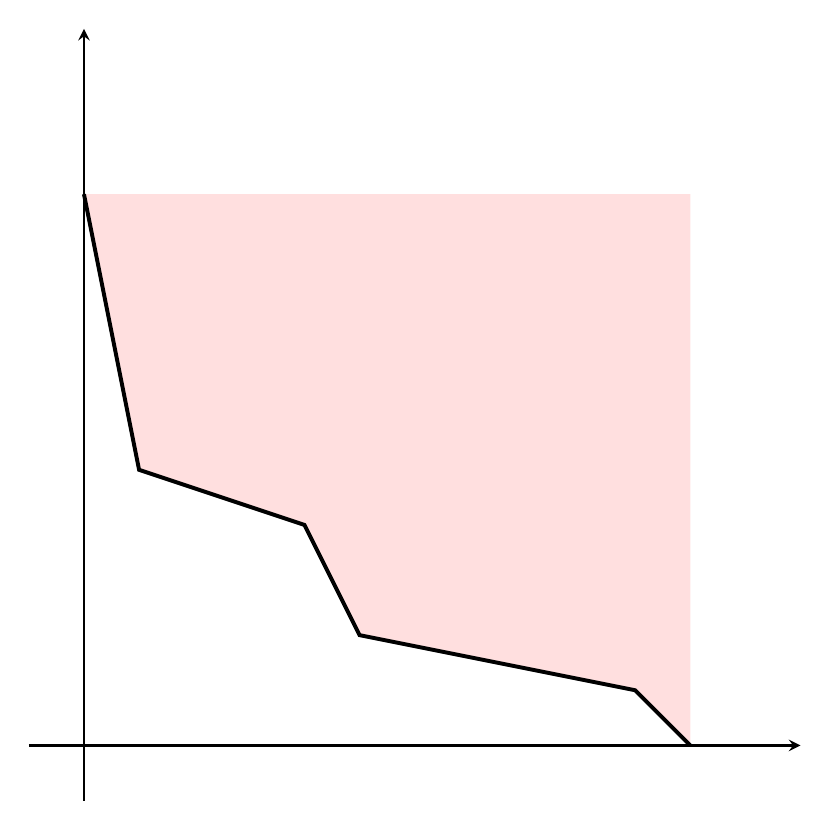
\begin{tikzpicture}[
        > = stealth, 
        line width = 0.3mm, 
        scale = 0.7
    ]
        \draw[fill = pink, fill opacity = 0.5, draw = none] (0,10) -- (1,5) -- (4,4) -- (5,2) -- (10,1) -- (11,0) -- (11,10) -- cycle;
        \draw[->] (-1,0) -- (13,0);
        \draw[->] (0,-1) -- (0,13);
        \draw[line width = 0.5mm] (0,10) -- (1,5) -- (4,4) -- (5,2) -- (10,1) -- (11,0);
    \end{tikzpicture}
    
    \caption{Một tập chuẩn đảo trong trường hợp hai chiều (được minh họa bằng phần màu hồng).}
    \label{fig:2}
\end{figure}

\begin{dn}[Tuy2000 \cite{Tuy2000}]
    Một tập $B \subset \R^p$ được gọi là một \textit{đa hộp (t.ư., đa hộp đảo)} trong hộp $[a, b]$ (t.ư., $[z, b]$), trong đó $z \in T$ và $T$ là một tập hữu hạn các đỉnh thuộc $[a, b]$.
\end{dn}

Khi đó ta gọi $T$ là tập đỉnh của đa hộp (t.ư., đa hộp đảo) $B$. Ta cũng
nói đa hộp (t.ư., đa hộp đảo) $B$ được sinh ra bởi $T$.

\begin{figure}[!h]
    \centering
    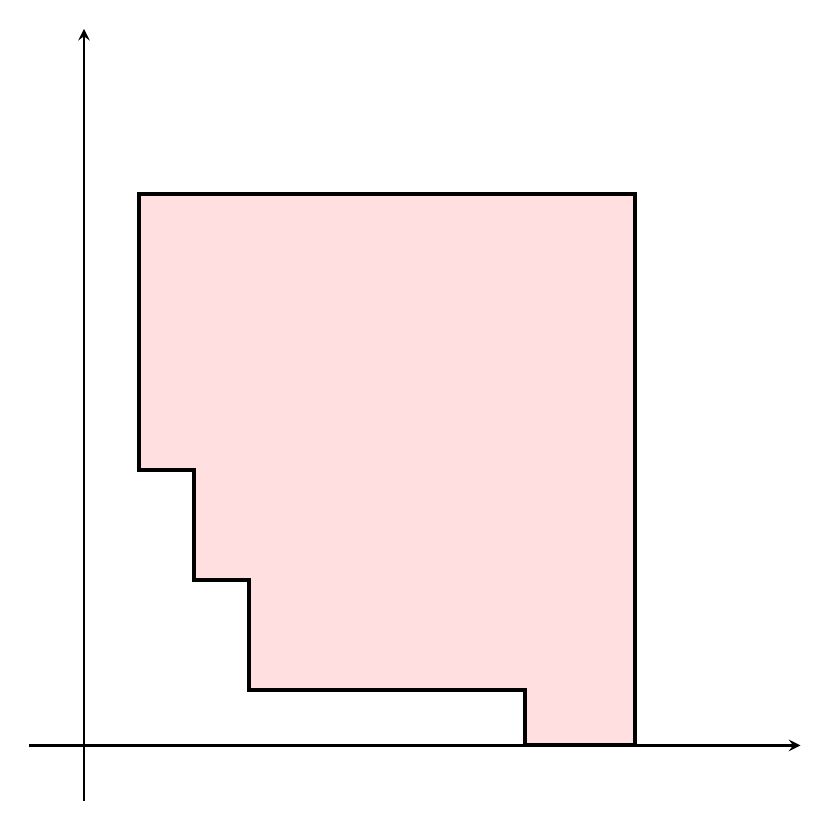
\begin{tikzpicture}[
        > = stealth, 
        line width = 0.3mm, 
        scale = 0.7
    ]
        \draw[fill = pink, fill opacity = 0.5, draw = none] (1,10) -- (1,5) -- (2,5) -- (2,3) -- (3,3) -- (3,1) -- (8,1) -- (8,0) -- (10, 0) -- (10, 10) -- cycle;
        \draw[->] (-1,0) -- (13,0);
        \draw[->] (0,-1) -- (0,13);
        \draw[line width = 0.5mm] (1,10) -- (1,5) -- (2,5) -- (2,3) -- (3,3) -- (3,1) -- (8,1) -- (8,0) -- (10, 0) -- (10, 10) -- cycle;
    \end{tikzpicture}
    \caption{ Một đa hộp đảo trong trường hợp hai chiều.}
    \label{fig:3}
\end{figure}

\begin{dn}[Tuy2000 \cite{Tuy2000}]
    Một đỉnh $z \in T$ được gọi là một đỉnh chính quy của đa hộp (t.ư., đa hộp đảo) $B$ nếu không tồn tại $z^\prime \in T, z^\prime \neq z$ sao cho $z^\prime$ (t.ư $z^\prime \leq z$). Hiển nhiên, một đỉnh $z \in T$ được gọi là \textit{không chính quy} khi nó không là đỉnh chính quy.
\end{dn}

\begin{md}[Tuy2000 \cite{Tuy2000}]
    Một đa hộp hoặc một đa hộp đảo được hoàn toàn xác định bởi các đỉnh chính quy của nó.
\end{md}

\begin{dl}[Tuy2000 \cite{Tuy2000}]
     Cho $f(x)$ là một hàm không giảm xác định trên đa hộp (t.ư., đa hộp đảo) $B$. Khi đó, $f(x)$ đạt giá trị cực đại (t.ư., cực tiểu) tại một đỉnh chính quy nào đó của $B$.
\end{dl}

\begin{md}[Tuy2000 \cite{Tuy2000}]
    Mọi đa hộp đều đóng và là tập chuẩn. Giao của một số hữu hạn các đa hộp là một đa hộp.
\end{md}
Mệnh đề sau đây chỉ ra cách xác định các đỉnh mới của một đa hộp đảo bằng kỹ thuật cắt đa hộp đảo được giới thiệu ở \cite{Tuy1999}
\begin{md}[Tuy 1999 \cite{Tuy1999}]
    Xét đa hộp đảo $[v, d]$ trong hộp $[b, d] \subset \R^p$ và một điểm $w$ thỏa mãn $v < w < d$. Khi đó tập $Q=[v, d] \setminus (w - int \R^p_+)$ là một đa hộp đảo có tập đỉnh được xác định như sau
    \begin{equation*}
        z^i = v + (w_i - v_i)e^i, \quad i = 1, \dots p,
    \end{equation*}
    trong đó $e$ là véc tơ đơn vị trong không gian $\R^p$
\end{md}

\begin{md} [Tuy 1999 \cite{Tuy1999}]
    \label{approx_normal_set}
     Có thể xấp xỉ một tập chuẩn (t.ư.,
tập chuẩn đảo) bằng một đa hộp (t.ư., đa hộp đảo) với một sai số nhỏ
bất kỳ.
\end{md}




